\subsubsection{Project : Creating new Projects}
	Once a user has been successfully authenticated by the UPRM system, the user should be able to create a new project. On creation of a new project, the user will have to provide the following details:
	\begin{itemize}
		\item Name(or Title) of the new project.
		\item A short description of the new project.
		\item An overall project deadline.
		\item Optional project specific sub-deadlines to track progress. The default timeline will be from project creation date to overall project deadline and a 1\% progress.
	\end{itemize}
	\textbf{Pre-Conditions}
	\begin{itemize}
		\item User has to be successfully authenticated.
	\end{itemize}
	\textbf{Post-Conditions}
	\begin{itemize}
		\item A new project should be created.
		\item The new project information should be saved in a database.
	\end{itemize}
	\textbf{Use case diagram for creation of projects: }\\
	\centerline{\fbox{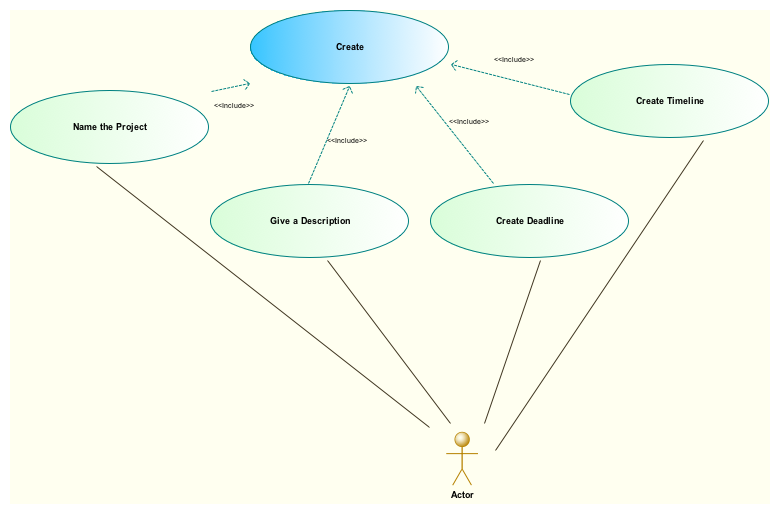
\includegraphics[width=\linewidth]{CRUD/uprm_create.png}}}
	
\subsubsection{Project : Creation of timeline}
	As soon as a project is created, a timeline for that project is also created. This timeline will be used by the statistics module and the users to track the progress of the project.\\
\textbf{Pre-Conditions}
\begin{itemize}
	\item User has to be successfully authenticated.
	\item A project has to exist. 
\end{itemize}
\textbf{Post-Conditions}
\begin{itemize}
	\item The starting date of the timeline should be saved.
	\item Optional sub-deadlines should be saved.
	\item A progress indicator (defaulting to 1\%) should be updated.
\end{itemize}
\textbf{Use case diagram for creation of timelines: }\\
\centerline{\fbox{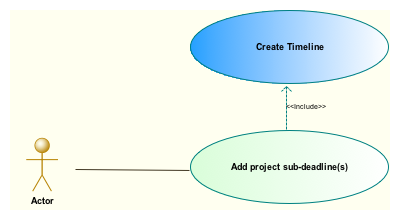
\includegraphics[scale=0.6]{CRUD/uprm_createTimeline.png}}}	
	
\subsubsection{Project : Updating of existing Projects}
	The user should be able to edit the details of an existing project. The user will not at any point be able to change the creation date of the project however the details the user will be able to change will be as follow:
	\begin{itemize}
		\item Name(or Title) of the project.
		\item The description of the project.
		\item The optional project specific sub-deadlines for progress tracking. This means adding and removing new sub-deadlines to the timeline.
	\end{itemize}
\textbf{Pre-Conditions}
\begin{itemize}
	\item User has to be successfully authenticated.
	\item User has to have the rights/permissions to the particular project.
	\item The project to be updated has to exist. 
\end{itemize}
\textbf{Post-Conditions}
\begin{itemize}
	\item The project details should be updated.
	\item The project information should be updated in a database.
	\item The progress indicator should be updated.
\end{itemize}
\textbf{Use case diagram for updating of projects: }\\
\centerline{\fbox{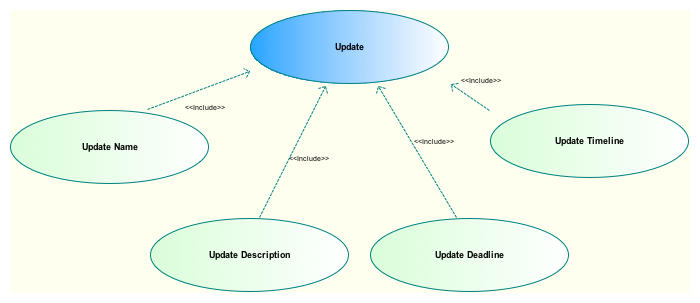
\includegraphics[width=\linewidth]{CRUD/uprm_update.png}}}

\subsubsection{Project : Updating of existing project timeline}
The user should be able to update the timeline of their project at any time. This meaning that the user should be able to add and remove sub-deadlines. This will impact the progress indicator.\\
\textbf{Pre-Conditions}
\begin{itemize}
	\item User should be successfully authenticated.
	\item A project has to exist.
	\item The user should have the rights/permissions to the particular project.
	\item A timeline for the particular project should exist.
\end{itemize}
\textbf{Post-Conditions}
\begin{itemize}
	\item The optional sub-deadlines should be updated in the database.
	\item The progress indicator should be updated.
\end{itemize}
\textbf{Use case diagram for updating of timelines: }\\
\centerline{\fbox{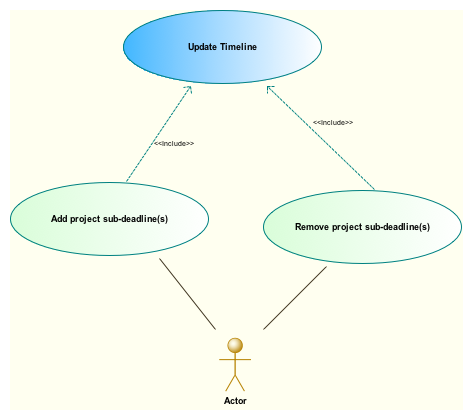
\includegraphics[scale=0.5]{CRUD/uprm_updateTimeline.png}}}

\subsubsection{Project : Deletion of existing project}
A user should be able to discard a project completely at any time. Once the user has chosen to delete a project, the project is completely removed from the UPRM system and all data regarding that project, removed from the UPRM system.\\
\textbf{Pre-Conditions}
\begin{itemize}
	\item User should be successfully authenticated.
	\item A project has to exist.
	\item The user should have the rights/permissions to the particular project.
\end{itemize}
\textbf{Post-Conditions}
\begin{itemize}
	\item The particular project information should be deleted from the database.
\end{itemize}
\textbf{Use case diagram for deleting of projects: }\\
\centerline{\fbox{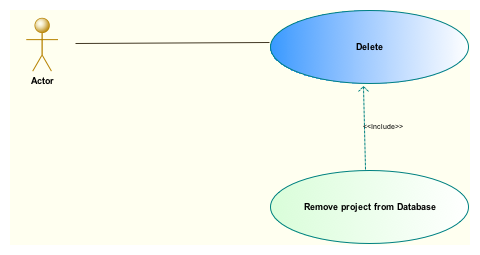
\includegraphics[scale=0.5]{CRUD/uprm_delete.png}}}